\section{Design and Implementation of \textsf{PCStream}}

\begin{figure}[b]
	\centering
	%\vspace{-10pt}
	%\includegraphics[width=0.6\linewidth]{figure/architecture4}
	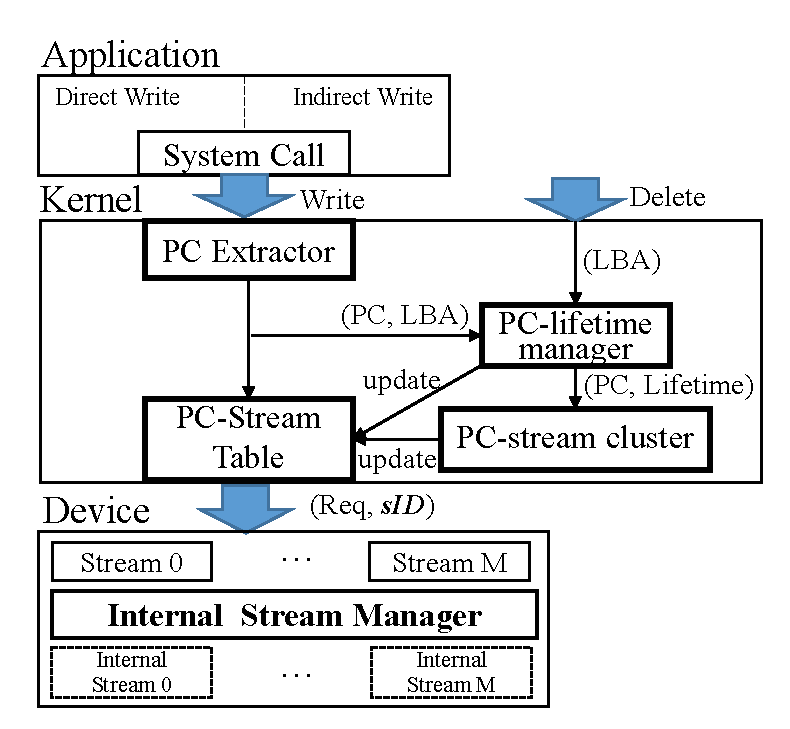
\includegraphics[width=0.6\linewidth]{figure/overview}
	%\vspace{-9pt}
	\caption{An overall architecture of \textsf{\small PCStream}.}
	\label{fig:architecture}
	%\vspace{-22pt}
\end{figure}

In this section, we explain the details of the proposed automatic stream
management technique, \textsf{\small PCStream}.
% COMMENT: maybe not necessary
%We first explain how we automatically extract PCs from applications at runtime
%and then describe how a large number of PCs are maintained in the DRAM memory
%and are mapped to a few streams available in an SSD.  Finally, we discuss
%design issues associated with the implementation of internal streams inside an
%SSD.
Fig.~\ref{fig:architecture} shows an overall organization of \textsf{\small
PCStream}. The \textit{PC extractor module} implemented as part of a system
call handler in the Linux kernel is responsible for computing \textit{a PC
signature}, which is used as a unique ID of each program context.  A PC
signature is obtained by summing program counter values~\cite{PC} along the
execution path to write-related system calls (e.g., {\tt write()}).  With a PC
signature, data written through specific call paths of applications can be
monitored at the program context level.  A PC signature is then delivered to
the \textit{PC-lifetime manager}, which caches collected PC signatures in the
memory and estimates expected lifetimes of data belonging to given PCs.  Since
product SSDs only expose a limited number of streams outside, the
\textit{PC-stream cluster} groups PCs with similar lifetimes using a mapping
policy. Data belonging to a same group have a same stream ID.

%the lifetime of data written by write-related system calls can be
%monitored at the program context level.  
%A PC signature value is stored in an
%inode data structure of a file system (modified for \textsf{\small PCStream})
%and is delivered to \textit{the lifetime analyzer module} which estimates
%expected lifetimes of data belonging to a given PC in the block device level.
%In order to efficiently detect the end of data lifetime in append-only
%workloads, the lifetime analyzer also intercepts TRIM~\cite{TRIM} requests from
%a file system.

%shane part Based on the lifetime information, \textit{the PC-to-stream mapper
%module} clusters PCs with similar lifetimes and maps them together to the same
%stream ID.  This mapping is required because the number of streams in an SSD
%is generally less than the number of PCs in host applications.

\subsection{Automatic PC computation}
As mentioned earlier, a PC signature defined to be the sum of program counter
values along the execution path of function calls that finally reaches a
write-related system function.  In theory, program counter values in the
execution path can be extracted in a relatively straightforward manner.  Except
for inline functions, every function call involves pushing the address of the
next instruction of a caller as a return address to the stack, followed by
pushing a frame pointer value.  In general, by referring to frame pointer
values, we are able to back-track stack frames of a process and selectively get
return addresses for generating a PC signature.  For example,
Fig.~\ref{fig:getpc}(a) shows an abstracted execution path of flushing data in
RocksDB, and Fig.~\ref{fig:getpc}(b) illustrates how a PC signature is obtained
by back-tracking the stack.  The return addresses are pushed before calling the
\textsf{\small  write()}, \textsf{\small  BuildTable()} and \textsf{\small
WriteLevel0Table()} functions.  Since frame pointer values in the stack hold
the addresses of previous frame pointers, we can easily obtain return addresses
and accumulate them to compute a PC signature.  

The frame pointer-based approach for computing a PC signature, however, is not
always possible because modern C/C++ compilers often do not use a frame pointer
for improving the efficiency of register allocation.  One example is a {\tt
-fomit-frame-pointer} option of GCC~\cite{GCC}.  This option allows the frame
pointer to be used as a general-purpose register, but makes it difficult for us
to back-track return addresses along the call chains.  

\begin{figure}[t]
%	\vspace{-10pt}
	\centering
	%\vspace{-8pt}
	\subfloat[An abstracted execution path for flushing data.]{\includegraphics[width=0.4\textwidth]{figure/getpc_1}}  
	%\vspace{-14pt}
	\hfill
	\subfloat[with the frame pointer.]{\includegraphics[width=0.22\textwidth]{figure/getpc_2}}
	\subfloat[without the frame pointer.]{\includegraphics[width=0.22\textwidth]{figure/getpc_3}}
	%\vspace{-9pt}
	%\caption{An example execution path and its PC extraction methods.}
	\caption{An example execution path and its PC extraction.} %shane part
	\label{fig:getpc}
	%\vspace{-20pt}
\end{figure}

The PC extractor of \textsf{\small PCStream} employs a simple but effective
workaround for back-tracking a call stack when a frame pointer is not
available.  When a write system call is made, the PC extractor scans every word
in the stack and checks if it belongs to process's code segment.  If the
scanned stack word holds a value within the address range of the code segment,
it assumes that it is a return address.  Since scanning the entire stack takes
too long, we stop the scanning when a sufficient number of return address
candidates are found. In the current implementation, only five candidates are
used for PC computation.  Even though it is quite ad-hoc, this restricted scan
is effective in distinguishing different PCs; it is very unlikely that two
different PCs follow exactly the same execution path to the \textsf{\small
write()} system call.  In our evaluation with a 3.4 GHz CPU machine, the
overhead of the restricted scan was almost negligible, taking only 300-400
$n$sec per \textsf{\small write()} system call.

\subsection{PC extraction for indirect writes}
One limitation of using PCs to extract I/O characteristics is that it only
works with C/C++ programs that \textit{directly} call write-related system
calls.  Many programs, however, often invoke write system calls
\textit{indirectly} through intermediate layers, which makes it difficult to
track program contexts.

The most representative example may be Java programs, such as Cassandra and
Hadoop, that run inside a Java Virtual Machine (JVM). Java programs invoke
write system calls via a native library written in C, so the PC extractor fails
to capture I/O activities of application logics because it is unable to see the
stack of Java programs.  Another example is C/C++ programs that use a write
buffer dedicated to dealing with writes from application logics. For example,
in MySQL~\cite{ref} and PostgreSQL~\cite{ref}, all the writes are first
destined for a write buffer, and then flush threads materialize buffered data
to persistent storage later.  In that case, the PC extractor only captures PCs
of flush threads since application logics run in other threads with different
stacks.

The problem of indirect writes can be addressed by collecting PC signatures at
the front-end interface of an intermediate layer that accepts write requests
from application logics. In case of Java programs, a native library can be
modified to capture write requests and computes PC signatures. Once a native
library is modified, it automatically gathers PC signatures without modifying
application code. Fig.~\ref{fig:java} illustrates how \textsf{PCStream}
collects signatures from Java programs.  \textcolor{red}{(TODO: Java 경우에
대한 그림과 설명이 추가되면 좋을 듯)}

Unlike Java, there is no a straightforward way to support PC collection for
applications with write buffers. This is because the implementation of write
buffering is different depending on applications, so additional efforts are
needed to manually modify code. However, this manual modification is only
limited to a write buffering module, and application logics themselves don't
need to be edited or annotated.




\subsection{PC lifetime management}
{\color{blue}Lifetime manager는 생성된 데이터의 수명을 계산하고 이를 PC 별로 구분하여 관리한다.
Lifetime Manager의 목적은 PC별 수명의 패턴을 파악하여 stream 할당의 기준을 만드는 것이다.
다양한 평가 결과, 우리는 동일한 I/O activity의 데이터라도 update 혹은 삭제 시기에 따라
개별적 데이터의 수명은 조금씩 달라지지만, 고유한 수명 패턴은 유지되는 것을 확인하였다.
따라서 lifetime manager는 수명의 정확한 값을 추구하기 보다는 수명의 대략적인 패턴을 파악하는 것을 목표로 한다.

데이터 lifetime은 쓰기 request가 issue된 때 부터 해당 주소가 다시 write되거나 
TRIM command에 의해 삭제될 때 까지로 정의된다.}
%The data lifetime of the append-only workload is defined 
%from when a write request is issued until the TRIM command~\cite{TRIM} is issued to 
%the corresponding address.
In order to measure the lifetime of data, the lifetime analyzer 
records the write time and PC value for each write request using its LBA.
Upon receiving the TRIM command or updating write request, the lifetime analyzer can compute the 
lifetime of the corresponding data using the recorded information.
{\color{blue} 
그러나 device 전체 LBA 공간에 대해 쓰여진 시간 정보를 유지하는 것은 메모리 부하가 크기 때문에,
우리는 1MB 크기의 chunk 단위로 나누어 관리하는 최적화 기법을 사용한다.
}
Note that, the
same PC may generate multiple data streams with different lifetimes.
We take the average lifetime as the PC's lifetime.

{\color{blue} Section 3에서 언급했듯이, PC는 user stack에 존재하는 
return address 즉, virtual address 기반으로 계산되므로
한 프로그램을 반복적으로 수행하면 동일한 PC들을 발견할 수 있다.
첫번째 수행 중 얻은 PC 별 lifetime 정보를 다음번 수행에서도 활용하기 위해 
이 정보를 유지하는 cache를 사용한다.
등장한 PC들과 그들의 lifetime 정보는 cache에 유지되고 추후 동일한 PC에 대해서는 
누적된 수명 정보를 활용할 수 있기 때문에 좀 더 정확한 수명 판단이 가능하다.
PC 값과 수명 값의 크기가 작기 때문에 몇십 KB의 메모리 만으로 충분히 많은 양의 데이터를 
유지할 수 있다. 따라서 본 논문에서는 PC cache replacement 정책에 대해서는 논의하지 않는다.
}

\subsection{Mapping PCs to SSD streams}

The last step in \textsf{\small PCStream} is to map
a group of PCs with similar lifetimes to an SSD stream.
This is because each SSD supports a limited number of stream IDs. For
example, SSDs used in \textsf{\small FStream}~\cite{FStream} and \textsf{\small AutoStream}~\cite{AutoStream}
support only 9 and 16 streams, respectively. 
{\color{blue} PC cluster는 비슷한 수준의 수명을 가진 PC들을 하나의 group으로 구분하기 위해 clustering algorithm을 사용한다.
본 연구에서는 overhead가 적고 많이 사용되는 k-means 알고리즘을 사용하였다.
SSD가 제공하는 stream의 개수와 동일한 group을 생성하여 각 PC group을 각 stream으로 할당한다.
}

%To properly group multiple PCs,
%the PC-to-stream mapper employs a simple 1-D clustering algorithm. 
%In order to cluster PCs with similar lifetimes, the mapper calculates the 
%lifetime difference between PCs.
%Then, PCs with the smallest lifetime difference are clustered into the same PC group. 
%The mapper repeats this clustering step until all the PCs are assigned to their PC groups.
{\color{blue} 추가로, SSD가 지원하는 stream의 개수가 변경되는 상황에서도 reclustering을 통해
대응이 가능하다.
For adapting to changing workloads, reclustering operations should be regularly performed. 
reclustering의 주기는 workload의 변화 패턴에 따라 결정될 수 있다.
새로운 PC가 계속적으로 생성되거나 한 PC의 수명 패턴이 자주 변화할 경우 reclustering의 주기를 
좀 더 짧게 설정하여 workload 변화를 반영한다.
}
%Since the
%number of PCs created by applications is not limited, the clustering algorithm
%must be efficient enough to quickly handle many PCs. 


